%%% LaTeX Template: Two column article
%%%
%%% Source: http://www.howtotex.com/
%%% Feel free to distribute this template, but please keep to referal to http://www.howtotex.com/ here.
%%% Date: February 2011

%%% Preamble
\documentclass[	DIV=calc,%
							paper=a4,%
							fontsize=11pt,%
			  ]{scrartcl}	 					% KOMA-article class

\usepackage{lipsum}													% Package to create dummy text

\usepackage[french]{babel}										% English language/hyphenation
\usepackage{courier}
\usepackage[protrusion=true,expansion=true]{microtype}				% Better typography
\usepackage{amsmath,amsfonts,amsthm}					% Math packages
\usepackage[pdftex]{graphicx}									% Enable pdflatex
\usepackage{moreverb}
\usepackage[margin=1in]{geometry}
\usepackage[svgnames]{xcolor}									% Enabling colors by their 'svgnames'
\usepackage[hang, small,labelfont=bf,up,textfont=it,up]{caption}	% Custom captions under/above floats
\usepackage{epstopdf}												% Converts .eps to .pdf
\usepackage{subfig}													% Subfigures
\usepackage{booktabs}
\usepackage{hyperref}												% Nicer tables
\usepackage{fix-cm}													% Custom fontsizes
\usepackage[utf8]{inputenc}
\usepackage[rightcaption]{sidecap} 
\usepackage{graphicx} %package to manage images
\usepackage{listings}
\usepackage{color}

\definecolor{mygreen}{rgb}{0,0.6,0}
\definecolor{mygray}{rgb}{0.5,0.5,0.5}
\definecolor{mymauve}{rgb}{0.58,0,0.82}

\lstdefinestyle{customc}{
  belowcaptionskip=1\baselineskip,
  breaklines=true,
  frame=L,
  xleftmargin=\parindent,
  language=bash,
  showstringspaces=false,
  basicstyle=\ttfamily,
  keywordstyle=\bfseries\color{green!40!black},
  commentstyle=\itshape\color{purple!40!black},
  %identifierstyle=\color{blue},
  stringstyle=\color{orange},
}


\lstset{escapechar=@,style=customc}

\lstset{ %
  language=bash,
  backgroundcolor=\color{white},   % choose the background color; you must add \usepackage{color} or \usepackage{xcolor}
%  basicstyle=\ttfamily,        % the size of the fonts that are used for the code
  basicstyle=\scriptsize\ttfamily,        % the size of the fonts that are used for
  breakatwhitespace=false,         % sets if automatic breaks should only happen at whitespace
  breaklines=true,                 % sets automatic line breaking
  captionpos=b,                    % sets the caption-position to bottom
  commentstyle=\color{mygreen},    % comment style
  deletekeywords={...},            % if you want to delete keywords from the given language
  escapeinside={\%*}{*)},          % if you want to add LaTeX within your code
  extendedchars=true,              % lets you use non-ASCII characters; for 8-bits encodings only, does not work with UTF-8
  frame=single,	                   % adds a frame around the code
  keepspaces=true,                 % keeps spaces in text, useful for keeping indentation of code (possibly needs columns=flexible)
  keywordstyle=\color{blue},       % keyword style
  otherkeywords={*,...},           % if you want to add more keywords to the set
  numbers=none,                    % where to put the line-numbers; possible values are (none, left, right)
  numbersep=5pt,                   % how far the line-numbers are from the code
  numberstyle=\tiny\color{mygray}, % the style that is used for the line-numbers
  rulecolor=\color{black},         % if not set, the frame-color may be changed on line-breaks within not-black text (e.g. comments (green here))
  showspaces=false,                % show spaces everywhere adding particular underscores; it overrides 'showstringspaces'
  showstringspaces=false,          % underline spaces within strings only
  showtabs=false,                  % show tabs within strings adding particular underscores
  stepnumber=2,                    % the step between two line-numbers. If it's 1, each line will be numbered
  stringstyle=\color{mymauve},     % string literal style
    belowskip=-3.3em,
  tabsize=2,	                   % sets default tabsize to 2 spaces
  title=\lstname                   % show the filename of files included with \lstinputlisting; also try caption instead of title
}



%%% Custom sectioning (sectsty package)
\usepackage{sectsty}													% Custom sectioning (see below)
\allsectionsfont{%															% Change font of al section commands
	\usefont{OT1}{phv}{b}{n}%										% bch-b-n: CharterBT-Bold font
	}

\sectionfont{%																% Change font of \section command
	\usefont{OT1}{phv}{b}{n}%										% bch-b-n: CharterBT-Bold font
	}



%%% Headers and footers
\usepackage{fancyhdr}												% Needed to define custom headers/footers
	\pagestyle{fancy}														% Enabling the custom headers/footers
\usepackage{lastpage}	

% Header (empty)
\lhead{}
\chead{}
\rhead{}
% Footer (you may change this to your own needs)
\lfoot{\footnotesize Thibaut EHLINGER et Benjamin HERB \textbullet ~ Internet des objets}
\cfoot{}
\rfoot{\footnotesize \thepage\ /\pageref{LastPage}}	% "Page 1 of 2"
\renewcommand{\headrulewidth}{0.0pt}
\renewcommand{\footrulewidth}{0.4pt}



%%% Creating an initial of the very first character of the content
\usepackage{lettrine}
\newcommand{\initial}[1]{%
     \lettrine[lines=3,lhang=0.3,nindent=0em]{
     				\color{DarkGoldenrod}
     				{\textsf{#1}}}{}}



%%% Title, author and date metadata
\usepackage{titling}															% For custom titles

\newcommand{\HorRule}{\color{DarkGoldenrod}%			% Creating a horizontal rule
									  	\rule{\linewidth}{1pt}%
										}
										
										\renewcommand\thesubsubsection{}

\pretitle{\vspace{-15pt} \begin{flushleft} \HorRule 
				\fontsize{15}{15} \usefont{OT1}{phv}{b}{n} \color{DarkRed} \selectfont 
				}
\title{TP IoT LAB}					% Title of your article goes here
\posttitle{\par\end{flushleft}\vskip 0.1em}

\preauthor{\begin{flushleft}
					\large \lineskip 0.1em \usefont{OT1}{phv}{b}{sl} \color{DarkRed}}
\author{Thibaut EHLINGER et Benjamin HERB }											% Author name goes here
\postauthor{\footnotesize \usefont{OT1}{phv}{m}{sl} \color{Black} 
					\newline Université de Strasbourg 								% Institution of author
					\par\end{flushleft}\HorRule}

\date{Mardi 13 décembre 2016}																			



%%% Begin document
\begin{document}
\maketitle
\thispagestyle{fancy} 			% Enabling the custom headers/footers for the first page 

% The first character should be within \initial{}
\initial{D}\textbf{ans} ce rapport, nous allons vous présenter notre travail concernant le TP2 d'IoT. Pour rappel, il fallait dans un premier temps modifier  certains paramètres (PanID, canal radio) et compiler une version de \texttt{Contiki OS} compatible avec les nœuds de la plate-forme FIT/IoT-lab. Ensuite il fallait flasher les six nœuds qui nous étaient attribués avec le binaire obtenu. Puis, nous avons dû : mettre en œuvre RPL ; analyser le déploiement du réseau avec le \textit{sniffer} Foren6 et étudier le \textit{Collect Tree Protocol (CTP)}.  Nous allons vous présenter les différentes étapes de ce TP.


\section{Contiki OS}
Contiki OS est un OS open source spécialisé dans les microcontrôleurs à basse consommation d'énergie reliés à un réseau. Dans un premier temps, nous avons modifié le code de Contiki OS. Pour modifier le canal il fallait modifier \texttt{RF2\_XX\_CHANNEL} dans le fichier \texttt{platform/openlab/radiorf2xx.c}. Nous lui avons affecté la valeur \textbf{17}. Pour le PanID, nous avons fait un \texttt{define IEEE802154\_CONF\_PANID} et nous avons utilisé l'ID \texttt{0x0007}, dans le fichier 
\texttt{contiki/platform/openlab/contiki-openlab-conf.h}.

Pour compiler Contiki OS, il fallait utiliser la commande \texttt{make} avec la bonne cible :
\begin{lstlisting}[language=bash]
$ make TARGET=iotlab-m3
\end{lstlisting}

Une fois le binaire généré, nous l'avons téléversé sur nos contrôleurs avec 
\begin{lstlisting}[language=bash]
$ node-cli -i 56476 -l strasbourg,m3,2+30-34 -up tutorial_m3.elf
\end{lstlisting}

\section{RPL}
Une fois nos contrôleurs dotés d'un OS, nous avons mis en œuvre RPL, un protocole de routage IPV6 prévu pour les WSN (\textit{Wireless sensor network}). RPL construit un DODAG (\textit{Destination Oriented Directed Acyclic Graph}) orienté vers le BR (\textit{Border router}) de notre réseau.

%TUTORIEL : https://www.iot-lab.info/tutorials/basic-m3-nodes-contiki-uip-stack-with-public-ipv6-on-ssh-front-end/

Pour information, notre sous-réseau a pour adresse IPv6 \texttt{2001:660:4701:f0a6/64}. Notre \textit{border-router} est le nœud numéro \textbf{\texttt{m3-2}}. Pour déployer notre réseau nous avons dû :
\begin{enumerate}
\item lancer \texttt{tunslip6} sur le serveur SSH ;
\begin{lstlisting}[language=bash]
$ sudo tunslip6.py 2001:660:4701:f0a6::1/64 -L -a m3-1 -p 20000
\end{lstlisting}
\item affecter au nœud \texttt{m3-2} son rôle de \textit{border-router} ;
\begin{lstlisting}[language=bash]
$ node-cli --update ~/border-router.iotlab-m3 -l strasbourg,m3,2
\end{lstlisting}
\item récupérer l'adresse du \textit{border-router}. Il s'agissait de \texttt{2001:660:4701:f0a6::a685}
\item déployer un serveur HTTP sur tous les autres nœuds du réseau :
\begin{lstlisting}[language=bash]
$ node-cli --update ~/http-server.iotlab-m3 -l strasbourg,m3,30-34
\end{lstlisting}
\end{enumerate}

Ci-dessous le texte lu sur l'interface web du BR :

\begin{lstlisting}
Neighbors
fe80::a786
fe80::b286
fe80::a885
fe80::b287
fe80::b086
Routes
2001:660:4701:f0a6::a786/128 (via fe80::a786) 16711327s
2001:660:4701:f0a6::b286/128 (via fe80::b286) 16711398s
2001:660:4701:f0a6::a885/128 (via fe80::a885) 16711398s
2001:660:4701:f0a6::b287/128 (via fe80::b287) 16711397s
2001:660:4701:f0a6::b086/128 (via fe80::b086) 16711396s
\end{lstlisting}

Et le texte lu sur l'un des autres nœuds :

\begin{lstlisting}
 Neighbors

fe80::a685 PREFERRED
fe80::b286
fe80::b287
fe80::b086
fe80::a885

Default Route

fe80::a685

Routes
\end{lstlisting}

\section{Foren6}
Dans cette section, nous allons déployer Foren6 sur l'un de nœuds de notre réseau dans le but de visualiser la construction du graphe RPL. Foren6 est un outil d'analyse non-intrusif de réseaux 6LowPan .
Pour visualiser les données, nous avons téléchargé et compilé le code issu du dépôt \url{https://github.com/cetic/foren6} :
\subsection{Mise en place de Foren6}
\begin{lstlisting}
$ sudo apt-get install libqt4-dev qt4-qmake cmake make libexpat1-dev tshark libpcap0.8-dev libc6-dev g++ gcc
$ git clone https://github.com/cetic/foren6.git
$ cd foren6
$ make run
\end{lstlisting}

Puis nous avons téléchargé le code de la partie Foren6 à exécuter sur le noeud. Avant de le compiler, il fallait modifier une ligne du code afin de configurer le bon canal radio :
\begin{lstlisting}[language=C]
// channel between 11 and 26
static uint8_t channel = 17;
\end{lstlisting}
Ensuite, nous avons compilé ce code spécifiquement pour les nœuds de la plateforme IoT-LAB :
\begin{lstlisting}[language=bash]
$ mkdir build.m3 && cd build.m3 && cmake .. -DPLATFORM=iotlab-m3
\end{lstlisting}

Il a fallu ensuite relier le \textit{sniffer} et l'interface graphique, puis relier le stream à un pseudo tty avec \texttt{socat} :

\begin{lstlisting}[language=C]
$ ssh -i /home/ben/.ssh/id_rsa 2016striot7@strasbourg.iot-lab.info -L 2001:m3-34:20000
$ socat TCP4:127.0.0.1:2001 pty,link=/tmp/mytty1,raw
\end{lstlisting}

Cela nous a permis d'obtenir une trace, dans \texttt{tty1}, pour visualiser notre graphe dans l'interface graphique Foren6.

\subsection{Utilisation de Foren6}
Nous avons d'abord \textit{flashé} le sniffer sur un nœud qui n'est pas notre BR (ici, le noeud \texttt{m30}) :

\begin{lstlisting}[language=bash]
$ node-cli -i 56200 -l strasbourg,m3,30 --update-profile sniffer
$ sniffer_aggregator -l strasbourg,m3,30 -o m3-30.pcap
\end{lstlisting}

Une fois la capture lancée, on \textit{reset} les nœuds, mise à part le \textit{sniffer}, afin d'être sûr que le \textit{sniffer} soit actif lors de l'initialisation du graphe.

\begin{lstlisting}[language=bash]
$ node-cli reset --exclude strasbourg,m30 
\end{lstlisting}

Malheureusement nous n'avons pas réussi à visualiser la topologie de notre réseau avec Foren6. Par conséquent, pour trouver notre PanID nous sommes passés par Wireshark. Comme prévu, c'était le \texttt{0x000007}.
La figure \ref{fig:wireshark} montre l'analyse de la capture avec Wireshark qui nous a permis de trouver notre PanID. La figure \ref{fig:script} nous montre l'exécution du script dans notre réseau. On y voit notre que notre graphe est composé d'une racine et de 5 feuilles, il n'y a donc aucun nœud intermédiaire dans notre topologie.

\begin{figure}
\centering
  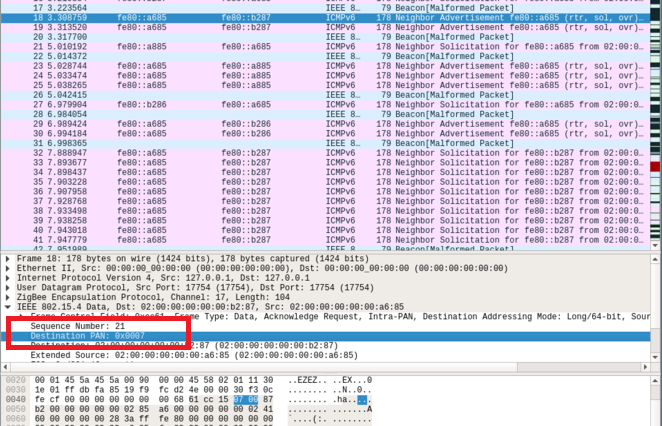
\includegraphics[keepaspectratio,width=\linewidth]{img/pan_id_720}
  \captionof{figure}{Pan ID (encadré rouge), trouvé grâce à Wireshark.}
  \label{fig:wireshark}
\end{figure}

\begin{figure}
\centering
  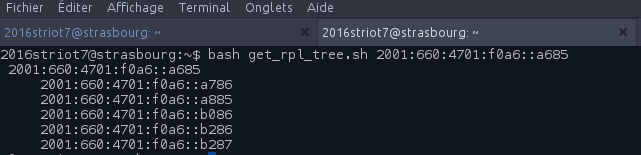
\includegraphics[keepaspectratio,width=\linewidth]{img/tree}
  \captionof{figure}{Exécution du script \texttt{get\_rpl\_tree.sh} dans notre réseau.}
  \label{fig:script}
\end{figure}

\section{Stack RIME}

Afin d'avoir un puit et cinq noeuds, nous avons compilé deux firmwares différents. Pour cela nous avons modifié example-collect.c. 

\begin{lstlisting}[language=C]
#DEFINE SINK 1

[...]

if(SINK) {
  printf("I am a sink\n");
  collect_set_sink(&tc, 1);
}
\end{lstlisting}

Pour créer le firmware \texttt{example-collect-sink.iotlab-m3} nous avons donc mis la valeur \texttt{SINK} à 1 et pour le firmware \texttt{example-collect-node.iotlab-m3} la valeur à 0.


Puis pour mettre en place une fréquence d'émission à 5 secondes, nous avons modifié cette partie de \texttt{example-collect.c} :

\begin{lstlisting}[language=C]
if(etimer_expired(&periodic)) {
  etimer_set(&periodic, CLOCK_SECOND * 5);
  etimer_set(&et, random_rand() % (CLOCK_SECOND * 5));
}
\end{lstlisting}

Enfin nous avons pu compiler puis flasher le firmware sur les différents noeuds :

\begin{lstlisting}[language=bash]
make TARGET=iotlab-m3

node-cli -i 56200 -l strasbourg,m3,30-34 -up example-collect-node.iotlab-m3 
node-cli -i 56200 -l strasbourg,m3,2 -up example-collect-sink.iotlab-m3 
\end{lstlisting}

\end{document}